\documentclass[11pt,letterpaper]{article}
\usepackage[utf8]{inputenc}
\usepackage{amsmath}
\usepackage{amsfonts}
\usepackage{amssymb}
\usepackage{fullpage}
\usepackage{hyphenat}
\usepackage{amsthm}

\usepackage{tikz}
\usetikzlibrary{arrows}
\usetikzlibrary{shapes.geometric}

\newcommand{\LP}{LINK PLACEMENT}
\newcommand{\HS}{HITTING SET}
\newcommand{\reals}{\mathbb{R}}

\newtheorem{lemma}{Lemma}

\begin{document}
\title{The Link Placement Problem}
\author{Bob West}
\maketitle

\section{Problem formulation}

We have:

- a hyperlink network $G=(V,E)$

- a set $P \subseteq V^*$ of navigation paths over this network

- after the navigation paths were collected, we introduce some previously non-existent links $E' \subseteq V^2 \setminus E$

- now, for each path $p=(p_1,\dots,p_n)$, we imagine that the user revisits the path step by step, and for each triple $(p_i,p_{i+1},p_{i+2})$ along the path for which $(p_i,p_{i+2}) \in E'$, the user has the option to choose the shortcut $(p_i,p_{i+2})$; i.e., in these cases the user may choose to skip over $p_{i+1}$

- we assume that, for each node triple $(s,m,t)$ with $(s,t) \in E'$, there is a fixed probability $q(s,m,t)$ with which the user will choose the shortcut $(s,t)$ over the full triple $(s,m,t)$

- this way, we can compute the probability of being chosen for each shortcut link along each path

- we emphasize that only single nodes can be skipped along a path, i.e., only forward\hyp  triangle\hyp closing operations are allowed in $G$

- consider a path $p=(p_1,\dots,p_n)$ and let $f^p_i$ be the probability that the (old) link $(p_i,p_{i+1})$ is clicked on path $p$, and $g^p_i$ the probability that the (new) link $(p_i,p_{i+2})$ is clicked

- define $x(s,t)$ as a binary variable indicating whether $(s,t) \in E'$

- then the above path\hyp specific probabilities are defined recursively as follows:

\begin{eqnarray}
\begin{array}{llll}
f^p_i &=& \left(f^p_{i-1} + g^p_{i-2}\right) \, (1 - x(p_i,p_{i+2}) \, q(p_i,p_{i+1},p_{i+2})) & \mbox{for $i=1,\dots,n-2$} \\
g^p_i &=& \left(f^p_{i-1} + g^p_{i-2}\right) \, x(p_i,p_{i+2}) \, q(p_i,p_{i+1},p_{i+2}) & \mbox{for $i=1,\dots,n-2$} \\
f^p_{i} &=& f^p_{i-1} + g^p_{i-2} & \mbox{for $i=n-1,n$} \\
f^p_0 &=& 1 & \\
g^p_{-1} &=& g^p_0 \;\;=\;\; g^p_{n-1} \;\;=\;\; g^p_n \;\;=\;\; 0 &
\end{array}
\label{eqn:f_and_g}
\end{eqnarray}

\begin{figure}
 \hspace*{-1.5cm}
 \centering
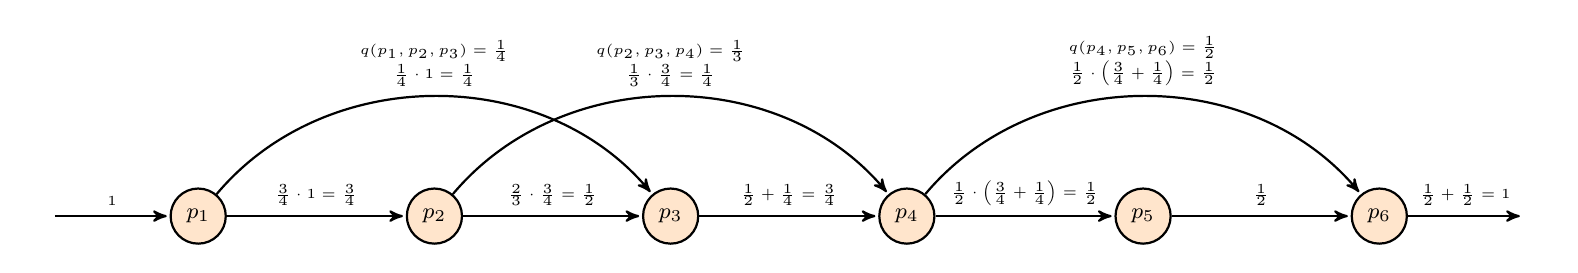
\begin{tikzpicture}[->,>=stealth',shorten >=1pt,auto,node distance=3cm,thick]

  \tikzstyle{p}=[circle,fill=orange!20,draw,font=\footnotesize,inner sep=0pt,minimum size=7mm]
  \tikzstyle{plain}=[circle,fill=white,font=\footnotesize]

  \node[plain] (p0) {};
  \node[p] (p1) [right of=p0, node distance=2cm] {$p_1$};
  \node[p] (p2) [right of=p1, node distance=3cm] {$p_2$};
  \node[p] (p3) [right of=p2, node distance=3cm] {$p_3$};
  \node[p] (p4) [right of=p3, node distance=3cm] {$p_4$};
  \node[p] (p5) [right of=p4, node distance=3cm] {$p_5$};
  \node[p] (p6) [right of=p5, node distance=3cm] {$p_6$};
  \node[plain] (p7) [right of=p6, node distance=2cm] {};
  \path[every node/.style={font=\tiny}]
    (p0) edge node {$1$} (p1)
    (p1) edge node {$\frac{3}{4}\cdot 1=\frac{3}{4}$} (p2)
    (p2) edge node {$\frac{2}{3}\cdot\frac{3}{4}=\frac{1}{2}$} (p3)
    (p3) edge node {$\frac{1}{2}+\frac{1}{4}=\frac{3}{4}$} (p4)
    (p4) edge node {$\frac{1}{2}\cdot\left(\frac{3}{4}+\frac{1}{4}\right)=\frac{1}{2}$} (p5)
    (p5) edge node {$\frac{1}{2}$} (p6)
    (p6) edge node {$\frac{1}{2}+\frac{1}{2}=1$} (p7);
  \path[every node/.style={font=\tiny}]
    (p1) edge [bend left=50] node[align=center] {$q(p_1,p_2,p_3)=\frac{1}{4}$\\$\frac{1}{4}\cdot 1=\frac{1}{4}$} (p3)
    (p2) edge [bend left=50] node[align=center] {$q(p_2,p_3,p_4)=\frac{1}{3}$\\$\frac{1}{3}\cdot\frac{3}{4}=\frac{1}{4}$} (p4)
    (p4) edge [bend left=50] node[align=center] {$q(p_4,p_5,p_6)=\frac{1}{2}$\\$\frac{1}{2}\cdot\left(\frac{3}{4}+\frac{1}{4}\right)=\frac{1}{2}$} (p6);

\end{tikzpicture}

\caption{...
}
 \label{fig:shortcut_example}
\end{figure}

- it follows that, if $(p_i,p_{i+2}) \notin E'$, then $g^p_i=0$

- flow interpretation: one unit of flow is transmitted from $p_1$ to $p_n$

- the flow that enters each node must equal the flow that leaves it

- each newly introduced shortcut link $(s,t) \in E'$ may appear in several paths, and has a probability of being clicked on each of these paths

- the value of that probability depends on the entire set $E'$ of new shortcut links

- by summing these probabilities for fixed $(s,t)$ across all paths, we obtain the number of clicks that shortcut is expected to receive

- so we can now phrase our optimization objective: given a budget of $K$ shortcut links that may be added, choose those shortcuts that would receive the maximum expected number of clicks

- more formally: we want to maximize $\sum_{p \in P} \sum_{i=1}^{|p|-2} g^p_i$, where $|p|$ is the number of nodes on path $p$.





\subsection{Integer linear program}

Note that in the above flow constraints (Eq.~\ref{eqn:f_and_g}), there is multiplicative interaction between the $f$ and $g$, and the $x$, variables.

It is nevertheless possible to formulate our optimization problem using only linear constraints (note that the $q$ terms are constants, while the $f$, $g$, and $x$ terms are optimization variables):

\begin{equation}
\text{maximize } \sum_{p \in P} \sum_{i=1}^{|p|-2} g^p_i \;\;\; \text{ subject to}
\label{eqn:ILP_objective}
\end{equation}

\begin{equation}
\begin{array}{rlll}
f^p_i + g^p_i &=& f^p_{i-1} + g^p_{i-2} & \mbox{for $i=1,\dots,n$} \\
g^p_i &\leq& x(p_i, p_{i+2}) & \mbox{for $i=1,\dots,n-2$} \\
g^p_i &\leq& \left(f^p_{i-1} + g^p_{i-2}\right) q(p_i,p_{i+1},p_{i+2}) & \mbox{for $i=1,\dots,n-2$} \\
f^p_0 &=& 1 & \\
g^p_{-1} &=& g^p_0 \;\;=\;\; g^p_{n-1} \;\;=\;\; g^p_n \;\;=\;\; 0 & \\
\sum_{(s,t) \in V^2} x(s,t) &\leq& K &  \\
x(s,t) &=& 0 & \mbox{for $(s,t) \in E$} \\
x(s,t) &\in& \{0,1\} & \mbox{for $(s,t) \in V^2$} \\
\end{array}
\label{eqn:ILP_constraints}
\end{equation}



\section{NP-hardness}

Integer linear programs are in general NP-hard, and here we show that this is also true for our case.

We proceed by reducing HITTING SET%
\footnote{Garey and Johnson, Problem SP8, p.~222}
to our problem.

First we formally define the LINK PLACEMENT and HITTING SET problems.

\subsection{Definition of the LINK PLACEMENT problem}

\begin{itemize}
\item INSTANCE: Directed graph $G=(V,E)$;
set of paths $P \subseteq V^*$;
positive integer $K$;
a shortcut probability for each node triple, i.e., a mapping $q : V^3 \rightarrow [0,1]$.
\item QUESTION: Given a budget of $K$ shortcut links $(s_1,t_1), \dots, (s_K,t_K)$, what is the maximum cumulative flow over the shortcuts across all paths, according to the model of Eq.~\ref{eqn:f_and_g}?
\end{itemize}

\subsection{Definition of the HITTING SET problem}

\begin{itemize}
\item INSTANCE: Collection $C$ of subsets of a finite set $Z$, positive integer $L \leq |Z|$.
\item QUESTION: Is there a subset $Z' \subseteq Z$ with $|Z'| \leq L$ such that $Z'$ contains at least one element from each subset in $C$?
\end{itemize}

Importantly, the problem remains NP-complete even if $|c| \leq 2$ for all $c \in C$.

\subsection{Reduction}

We need to reduce a HITTING SET instance $(C,Z,L)$ to a LINK PLACEMENT instance $(V,E,P,q,K)$.
We assume w.l.o.g.\ that each $c \in C$ contains at most two elements.

First, we construct the hyperlink network $G=(V,E)$.
For each $z_i \in Z$ we include three nodes $s_i,m_i,t_i$ in the hyperlink network:
\begin{equation}
V=\bigcup_{i=1}^{|Z|} \{s_i, m_i, t_i\}.
\end{equation}

Next, we construct the set $P$ of paths over these nodes. We construct one path per subset $c \in C$:
if $c=\{z_j,z_k\}$, we add the path $(s_j,s_k,t_j,t_k)$, and if $c=\{z_j\}$, we add the path $(s_j,m_j,t_j)$:
\begin{equation}
P = \bigcup_{\{z_j,z_k\} \in C} \{(s_j, s_k, t_j, t_k)\} \cup \bigcup_{\{z_j\} \in C} \{(s_j, m_j, t_j)\}.
\end{equation}

The edge set $E$ of $G$ is now simply defined as the set of edges induced by $P$:
\begin{equation}
E = \bigcup_{\{z_j,z_k\} \in C} \{(s_j,s_k), (s_k,t_j), (t_j,t_k)\} \cup \bigcup_{\{z_j\} \in C} \{(s_j,m_j), (m_j,t_j)\}.
\end{equation}

The probability of taking a shortcut, in the case it exists, is set to 1 for all shortcut candidates:
\begin{equation}
q(s,m,t) = 1, \;\;\;\; \mbox{for all $(s,m,t) \in V^3$}.
\end{equation}

And finally,
\begin{equation}
K=L.
\end{equation}


\begin{figure}
 \centering
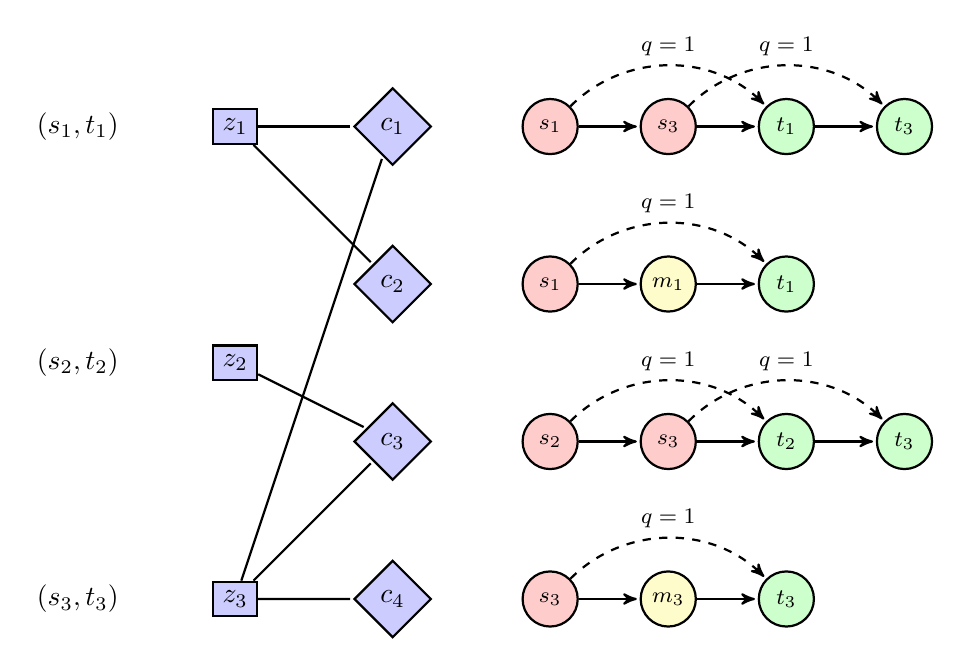
\begin{tikzpicture}[-,>=stealth',shorten >=1pt,auto,node distance=3cm,thick]

  \tikzstyle{plain}=[]
  \tikzstyle{elem}=[rectangle,fill=blue!20,draw]
  \tikzstyle{subset}=[diamond,fill=blue!20,draw]
  \tikzstyle{s}=[circle,fill=red!20,draw,font=\footnotesize,inner sep=0pt,minimum size=7mm]
  \tikzstyle{m}=[circle,fill=yellow!20,draw,font=\footnotesize,inner sep=0pt,minimum size=7mm]
  \tikzstyle{t}=[circle,fill=green!20,draw,font=\footnotesize,inner sep=0pt,minimum size=7mm]

  \node[elem] (u1) {$z_1$};
  \node[elem] (u2) [below of=u1] {$z_2$};
  \node[elem] (u3) [below of=u2] {$z_3$};

  \node[plain] (st1) [left of=u1, node distance=2cm] {$(s_1,t_1)$};
  \node[plain] (st2) [below of=st1] {$(s_2,t_2)$};
  \node[plain] (st3) [below of=st2] {$(s_3,t_3)$};

  \node[subset] (c1) [right of=u1, node distance=2cm] {$c_1$};
  \node[subset] (c2) [below of=c1, node distance=2cm] {$c_2$};
  \node[subset] (c3) [below of=c2, node distance=2cm] {$c_3$};
  \node[subset] (c4) [below of=c3, node distance=2cm] {$c_4$};

  \path[every node/.style={font=\small}]
    (u1) edge (c1)
    (u3) edge (c1)
    (u1) edge (c1)
    (u1) edge (c2)
    (u2) edge (c3)
    (u3) edge (c3)
    (u3) edge (c4);

  \node[s] (p11) [right of=c1, node distance=2cm] {$s_1$};
  \node[s] (p12) [right of=p11, node distance=1.5cm] {$s_3$};
  \node[t] (p13) [right of=p12, node distance=1.5cm] {$t_1$};
  \node[t] (p14) [right of=p13, node distance=1.5cm] {$t_3$};
  \path[->]
    (p11) edge (p12)
    (p12) edge (p13)
    (p13) edge (p14);
  \path[->,every node/.style={font=\footnotesize}]
    (p11) edge [bend left=45, dashed] node {$q=1$} (p13)
    (p12) edge [bend left=45, dashed] node {$q=1$} (p14);

  \node[s] (p21) [right of=c2, node distance=2cm] {$s_1$};
  \node[m] (p22) [right of=p21, node distance=1.5cm] {$m_1$};
  \node[t] (p23) [right of=p22, node distance=1.5cm] {$t_1$};
  \path[->]
    (p21) edge (p22)
    (p22) edge (p23);
  \path[->,every node/.style={font=\footnotesize}]
    (p21) edge [bend left=45, dashed] node {$q=1$} (p23);

  \node[s] (p31) [right of=c3, node distance=2cm] {$s_2$};
  \node[s] (p32) [right of=p31, node distance=1.5cm] {$s_3$};
  \node[t] (p33) [right of=p32, node distance=1.5cm] {$t_2$};
  \node[t] (p34) [right of=p33, node distance=1.5cm] {$t_3$};
  \path[->]
    (p31) edge (p32)
    (p32) edge (p33)
    (p33) edge (p34);
  \path[->,every node/.style={font=\footnotesize}]
    (p31) edge [bend left=45, dashed] node {$q=1$} (p33)
    (p32) edge [bend left=45, dashed] node {$q=1$} (p34);

  \node[s] (p41) [right of=c4, node distance=2cm] {$s_3$};
  \node[m] (p42) [right of=p41, node distance=1.5cm] {$m_3$};
  \node[t] (p43) [right of=p42, node distance=1.5cm] {$t_3$};
  \path[->]
    (p41) edge (p42)
    (p42) edge (p43);
  \path[->,every node/.style={font=\footnotesize}]
    (p41) edge [bend left=45, dashed] node {$q=1$} (p43);

\end{tikzpicture}

\caption{The reduction from HITTING SET to LINK PLACEMENT.
{\bf Blue:} the HITTING SET instance.
{\bf Red/yellow/green:} the paths constructed for the LINK PLACEMENT instance.
}
 \label{fig:reduction}
\end{figure}

The reduction is schematized in Fig.~\ref{fig:reduction}.
We now prove that by optimizing the \LP{} instance we could decide the \HS{} instance.
Therefore, \LP{} is at least as hard as \HS{}, which makes \LP{} NP-hard, since \HS{} is NP-complete.

In particular, we show that in the \HS{} instance we can hit all $|C|$ subsets with at most $K$ elements from $Z$ if and only if in the \LP{} instance the maximum shortcut flow that can be achieved by adding at most $K$ new shortcut edges is $|C|$.
The \HS{} instance could then be decided by computing the maximum for the \LP{} instance and checking if that maximum equals $|C|$.

The above equivalence can easily be verified in the sketch from Fig.~\ref{fig:reduction}.
Choosing $z_i$ in the \HS{} instance corresponds to introducing the shortcut $(s_i,t_i)$ in the \LP{} instance, and hitting subset $c$ corresponds to having at least one shortcut link available in the path corresponding to $c$.
Further, given the interleaving way in which the paths are constructed, and since all shortcut probabilities are 1, exactly one shortcut will be traversed in every path with at least one shortcut.
Hence, if all $|C|$ subsets can be hit in \HS{}, then the maximum shortcut flow is $|C|$ in \LP{}, and {\it vice versa}.



\section{Approximate solution via submodularity}

Let $\phi : 2^{V \times V} \rightarrow \reals$ be the function that computes the value of a solution to the link prediction problem, i.e., $\phi$ computes the cumulative flow over all shortcut edges.

In this section we show that $\phi$ is monotone submodular, which implies that it admits a $(1-1/e)$-approximation via greedy marginal\hyp gain optimization.

We use $\phi_p(E')$ to denote the value of the solution $E'$ when discarding all paths but $p$. The total value $\phi(E')$ is then obtained by summing over all path-wise values, i.e., $\phi(E') = \sum_{p \in P} \phi_p(E')$.

\begin{lemma}
\label{thm:monotonicity}
$\phi$ is monotone decreasing, i.e., $\phi(B) \leq \phi(A)$ if $A \subseteq B$.
\end{lemma}

\begin{proof}[Proof]
Without loss of generality, we need to consider only the case where $B$ is one element larger than $A$, i.e., $B = A \cup \{y\}$; the lemma will then follow by transitivity. Further, we may consider only the path-wise value $\phi_p$; the lemma will then also hold for $\phi$.
First, note that the flow over all edges upstream (i.e., towards the left in Fig.~\ref{fig:shortcut_example}) of $y$ will be unaffected when introducing $y$.
\end{proof}


\end{document}
